\documentclass[11pt,a4paper]{article}

% ---------- Fonts (premium: XCharter + Source Sans + Source Code Pro) ----------
\usepackage[T1]{fontenc}
\usepackage[utf8]{inputenc}
\usepackage[scaled=1.02]{XCharter}
\usepackage[semibold,scaled=0.94]{sourcesanspro}
\usepackage[scaled=0.82]{sourcecodepro}
\usepackage{textcomp}
\usepackage{amsmath}
\usepackage{microtype}

% ---------- Unicode passthrough so the source stays readable ----------
\usepackage{newunicodechar}
\newunicodechar{→}{\ensuremath{\rightarrow}}
\newunicodechar{←}{\ensuremath{\leftarrow}}
\newunicodechar{≤}{\ensuremath{\leq}}
\newunicodechar{≥}{\ensuremath{\geq}}
\newunicodechar{×}{\ensuremath{\times}}
\newunicodechar{−}{\textminus}
\newunicodechar{—}{\textemdash}
\newunicodechar{–}{\textendash}
\newunicodechar{“}{``}
\newunicodechar{”}{''}
\newunicodechar{‘}{`}
\newunicodechar{’}{'}
\newunicodechar{…}{\ldots}

% ---------- Layout ----------
\usepackage[a4paper,top=2.4cm,bottom=2.4cm,left=2.5cm,right=2.5cm]{geometry}
\usepackage{graphicx}
\usepackage{float}
\usepackage{enumitem}
\usepackage{booktabs}
\usepackage{tabularx}
\usepackage{array}
\usepackage{ragged2e}
\usepackage{colortbl}
\usepackage{caption}
\usepackage{titlesec}
\usepackage{fancyhdr}
\usepackage[section]{placeins}
\usepackage{xspace}
\usepackage[most]{tcolorbox}
\usepackage{tikz}
\usetikzlibrary{arrows.meta,positioning,calc,fit,backgrounds,shapes.geometric,
  decorations.pathreplacing,shadows.blur,shapes.multipart}

% ---------- Palette ----------
\definecolor{ink}{HTML}{1B2430}
\definecolor{inksoft}{HTML}{55606E}
\definecolor{accent}{HTML}{2F5C9E}   % blue  - read/used
\definecolor{green}{HTML}{3E8E5A}    % green - checked vs fixed value
\definecolor{amber}{HTML}{C08A1E}    % amber - files / capture
\definecolor{red}{HTML}{B03A3A}      % red   - attacker / deauth
\definecolor{gray}{HTML}{8A929C}     % gray  - present but unused
\definecolor{rule}{HTML}{2F5C9E}
\definecolor{pageband}{HTML}{EEF2F8}

\color{ink}
\linespread{1.06}

% ---------- Section styling ----------
\titleformat{\section}
  {\sffamily\bfseries\large\color{ink}}
  {\color{accent}\thesection\hspace{0.6em}}{0pt}
  {}[\vspace{2pt}{\color{rule}\titlerule[1pt]}]
\titleformat{\subsection}
  {\sffamily\bfseries\normalsize\color{accent!92!black}}
  {\thesubsection\hspace{0.5em}}{0pt}{}
\titleformat{\subsubsection}
  {\sffamily\bfseries\normalsize\color{ink}}
  {}{0pt}{}
\titlespacing*{\section}{0pt}{16pt}{7pt}
\titlespacing*{\subsection}{0pt}{11pt}{3pt}
\titlespacing*{\subsubsection}{0pt}{9pt}{2pt}

% ---------- Captions ----------
\captionsetup{font=small,labelfont={sf,bf,color=rule},textfont={sf},
  labelsep=period,skip=6pt,width=0.94\textwidth}

% ---------- Lists ----------
\setlist[itemize]{leftmargin=1.35em,itemsep=2.5pt,topsep=3pt,parsep=0pt}
\setlist[enumerate]{leftmargin=1.5em,itemsep=2.5pt,topsep=3pt}

% ---------- Tables ----------
\renewcommand{\arraystretch}{1.28}
\newcolumntype{L}[1]{>{\RaggedRight\arraybackslash}p{#1}}
\newcommand{\thd}[1]{\sffamily\bfseries\small\color{ink}#1}

% ---------- Header / footer ----------
\pagestyle{fancy}\fancyhf{}
\renewcommand{\headrulewidth}{0pt}
\fancyfoot[C]{\sffamily\footnotesize\color{inksoft}CSE406 — Topic 20 — WPA2 Handshake Capture, Offline Dictionary Attack \& WPA3-SAE Defense \;\textbullet\; Design Report}
\fancyfoot[R]{\sffamily\footnotesize\color{inksoft}\thepage}

% ---------- Inline helpers ----------
\newcommand{\code}[1]{{\ttfamily\small #1}}
\newcommand{\ra}{\ensuremath{\rightarrow}\xspace}
\usepackage{pifont}
\newcommand{\yes}{\textcolor{green}{\ding{51}}}
\newcommand{\dash}{\textcolor{gray}{\rule[0.35ex]{0.7em}{0.9pt}}}

% ---------- Console + callout boxes ----------
\newtcolorbox{console}{colback=ink!4,colframe=ink!22,boxrule=0.6pt,arc=2pt,
  left=8pt,right=8pt,top=5pt,bottom=5pt,fontupper=\ttfamily\scriptsize,
  before skip=6pt,after skip=6pt}
\newtcolorbox{whybox}{enhanced,colback=accent!5,colframe=accent!55,boxrule=0pt,
  leftrule=2.6pt,arc=1pt,left=10pt,right=10pt,top=7pt,bottom=7pt,
  before skip=8pt,after skip=8pt}

% ---------- Shared TikZ styles ----------
\tikzset{
  box/.style={draw,line width=0.8pt,rounded corners=3pt,align=center,inner sep=6pt},
  bRead/.style ={box,fill=accent!11,draw=accent!85!black,text=ink},
  bChk/.style  ={box,fill=green!14,draw=green!72!black,text=ink},
  bAmber/.style={box,fill=amber!16,draw=amber!85!black,text=ink},
  bRed/.style  ={box,fill=red!11,draw=red!78!black,text=ink},
  bOff/.style  ={box,fill=gray!16,draw=gray!85!black,text=ink},
  lbl/.style={font=\sffamily\scriptsize,text=inksoft,align=center},
  flow/.style={-{Stealth[length=3mm]},line width=1pt,draw=ink},
  flowred/.style={-{Stealth[length=2.6mm]},line width=1pt,draw=red!80!black,dashed},
  flowdot/.style={-{Stealth[length=2.6mm]},line width=1pt,draw=accent,densely dotted},
}

\usepackage[hidelinks,pdfusetitle]{hyperref}
\hypersetup{pdftitle={WPA2 Handshake Capture, Offline Dictionary Attack and WPA3-SAE Defense — Design Report},
  pdfauthor={CSE406 Topic 20 Group — 2105031, 2105057}}

% ============ editable group members ============
\newcommand{\groupmembers}{%
  \begin{tabular}{@{}L{6.9cm}@{}L{3.2cm}@{}}
    \thd{Name} & \thd{Student ID} \\[1pt]
    Nabiha Tahseen & \textcolor{inksoft}{2105031} \\
    Md.\ Mosharaf Hossain Apurbo & \textcolor{inksoft}{2105057} \\
  \end{tabular}}
\newcommand{\supervisorblock}{%
  {\sffamily\small\bfseries\color{ink}SUPERVISOR}\\[7pt]
  {\normalsize Imtiaz Kabir}\\[2pt]
  {\footnotesize\color{inksoft}Lecturer, Department of Computer Science and Engineering, BUET}}
% =================================================


% ---------- truth-table cell helpers ----------
\newcommand{\bit}[1]{{\sffamily\bfseries\color{accent}#1}}
\newcommand{\bz}{{\sffamily\color{gray}0}}
\newcommand{\dsh}{\textcolor{gray}{\textendash}}

% ---------- figure-specific TikZ styles ----------
\tikzset{
  % frame-layout (Fig 3)
  fR/.style={draw=accent!85!black,fill=accent!11,line width=0.8pt,rounded corners=2.5pt,minimum height=1.05cm,align=center,inner sep=2pt,font=\footnotesize,text=ink},
  fG/.style={draw=green!72!black,fill=green!15,line width=0.8pt,rounded corners=2.5pt,minimum height=1.05cm,align=center,inner sep=2pt,font=\footnotesize,text=ink},
  fO/.style={draw=gray!85!black,fill=gray!16,line width=0.8pt,rounded corners=2.5pt,minimum height=1.05cm,align=center,inner sep=2pt,font=\footnotesize,text=ink},
  ofl/.style={font=\sffamily\scriptsize,text=inksoft,align=center},
  sect/.style={font=\sffamily\bfseries\small,text=ink,anchor=south west},
  fn/.style={font=\ttfamily\scriptsize,text=accent!85!black},
  % bitfield (Fig 4)
  kR/.style={draw=accent!85!black,fill=accent!11,line width=0.8pt,rounded corners=2.5pt,minimum height=1.35cm,align=center,inner sep=2pt,font=\footnotesize,text=ink},
  kO/.style={draw=gray!85!black,fill=gray!16,line width=0.8pt,rounded corners=2.5pt,minimum height=1.35cm,align=center,inner sep=2pt,font=\footnotesize,text=ink},
  bitl/.style={font=\sffamily\scriptsize,text=inksoft},
  % flowchart (Fig 5)
  fclr/.style={draw,line width=0.9pt,rounded corners=3pt,align=center,inner sep=6pt,font=\small},
  cfg/.style ={fclr,fill=accent!7,draw=ink!55,text=ink},
  snif/.style={fclr,fill=amber!16,draw=amber!85!black,text=ink},
  deau/.style={fclr,fill=red!10,draw=red!75!black,text=ink},
  capf/.style={fclr,fill=amber!12,draw=amber!85!black,text=ink},
  hs/.style  ={fclr,fill=accent!11,draw=accent!85!black,text=ink},
  cr/.style  ={fclr,fill=green!13,draw=green!68!black,text=ink},
  cbox/.style={fclr,fill=green!15,draw=green!68!black,text=ink,font=\footnotesize,minimum height=1.25cm},
  term/.style={fclr,fill=gray!14,draw=gray!80!black,text=ink},
  dia/.style ={draw,line width=0.9pt,fill=amber!16,draw=amber!85!black,align=center,
               shape=diamond,aspect=2.2,inner sep=1pt,font=\small,text=ink},
  fg/.style={-{Stealth[length=2.6mm]},line width=1pt,draw=green!60!black},
}

% ================= FIGURE 1 : TOPOLOGY =================
\newcommand{\FIGONE}{%
\begin{figure}[!htb]\centering
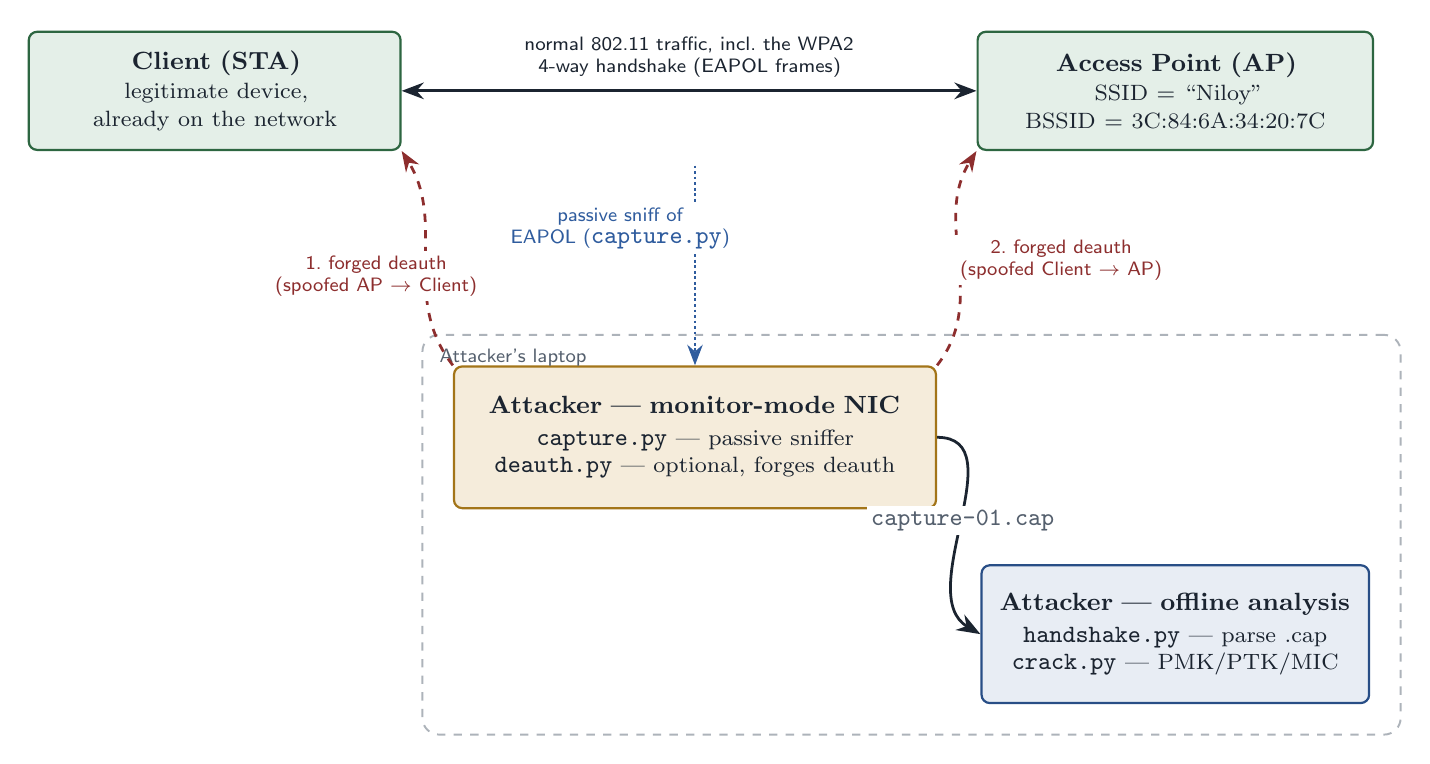
\begin{tikzpicture}[font=\small,node distance=0pt]
  \node[bChk,text width=4.3cm,minimum height=1.5cm] (client)
        at (0,4.7) {\textbf{Client (STA)}\\[1pt]\footnotesize legitimate device,\\[-1pt]\footnotesize already on the network};
  \node[bChk,text width=4.6cm,minimum height=1.5cm] (ap)
        at (12.2,4.7) {\textbf{Access Point (AP)}\\[1pt]\footnotesize SSID = ``Niloy''\\[-1pt]\footnotesize BSSID = 3C:84:6A:34:20:7C};
  \draw[{Stealth[length=2.8mm]}-{Stealth[length=2.8mm]},line width=1.1pt,draw=ink]
        (client.east) -- node[above,lbl,text=ink,yshift=1pt,align=center,text width=6.4cm]{normal 802.11 traffic, incl.\ the WPA2 4-way handshake (EAPOL frames)} (ap.west);
  \node[bAmber,text width=5.7cm,minimum height=1.8cm] (nic) at (6.1,0.3)
        {\textbf{Attacker --- monitor-mode NIC}\\[2pt]\footnotesize \code{capture.py} --- passive sniffer\\[-1pt]\footnotesize \code{deauth.py} --- optional, forges deauth};
  \node[bRead,text width=4.5cm,minimum height=1.75cm] (off) at (12.2,-2.2)
        {\textbf{Attacker --- offline analysis}\\[2pt]\footnotesize \code{handshake.py} --- parse .cap\\[-1pt]\footnotesize \code{crack.py} --- PMK/PTK/MIC};
  \begin{scope}[on background layer]
    \node[draw=gray!70,dashed,line width=0.7pt,rounded corners=6pt,
          fit=(nic)(off),inner sep=11pt] (lap) {};
  \end{scope}
  \node[lbl,anchor=north west,text=inksoft] at ([xshift=3pt,yshift=-2pt]lap.north west) {Attacker's laptop};
  \draw[flowdot] (6.1,3.75) -- (nic.north);
  \node[lbl,text=accent,fill=white,inner sep=1.8pt,align=center] at (5.15,2.95)
        {passive sniff of\\ EAPOL (\code{capture.py})};
  \draw[flowred] (nic.north west) to[out=128,in=-58] (client.south east);
  \node[lbl,text=red!80!black,fill=white,inner sep=1.8pt,align=center] at (2.05,2.35)
        {1.\ forged deauth\\ (spoofed AP $\rightarrow$ Client)};
  \draw[flowred] (nic.north east) to[out=52,in=-122] (ap.south west);
  \node[lbl,text=red!80!black,fill=white,inner sep=1.8pt,align=center] at (10.75,2.55)
        {2.\ forged deauth\\ (spoofed Client $\rightarrow$ AP)};
  \draw[flow] (nic.east) to[out=0,in=150] node[lbl,fill=white,inner sep=1.5pt,pos=0.5]{\code{capture-01.cap}} (off.west);
\end{tikzpicture}
\caption{Network topology. The attacker plays two separate roles: an on-air sniffer/injector and a purely offline analysis stage. Steps~1--2 (\code{deauth.py}) are optional --- sniffing and cracking still work if the client reconnects naturally, it just takes longer to wait for.}
\label{fig:topology}
\end{figure}}

% ================= FIGURE 2 : TIMING =================
\newcommand{\FIGTWO}{%
\begin{figure}[!htb]\centering
\resizebox{\textwidth}{!}{%
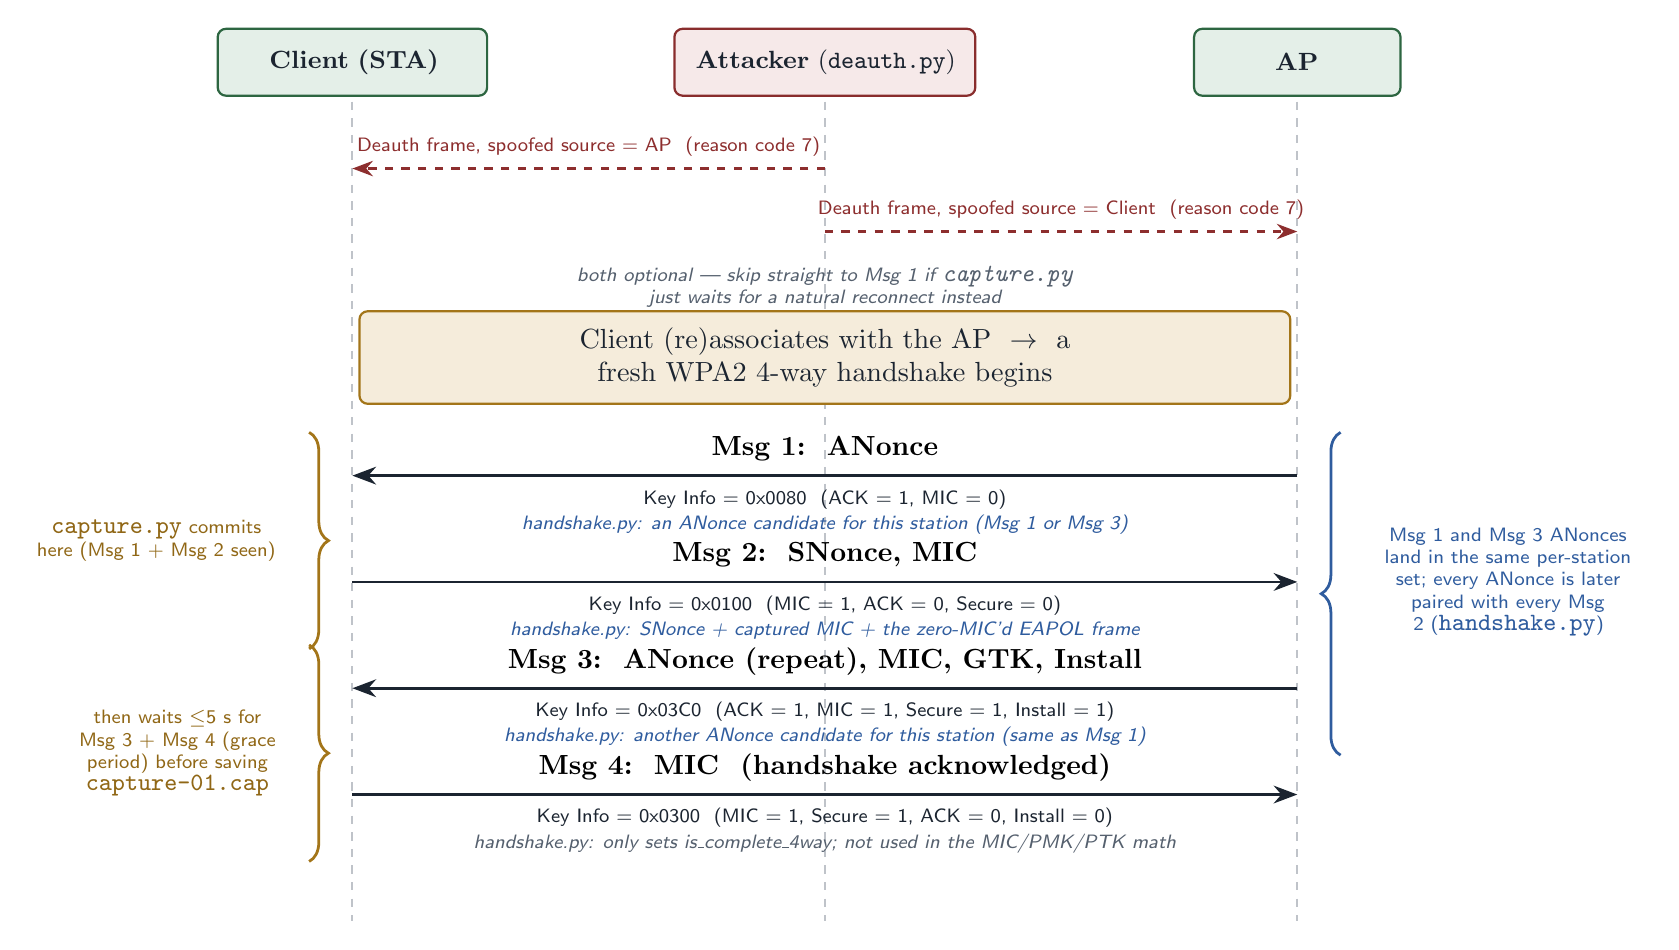
\begin{tikzpicture}[font=\small]
  \def\sta{0}\def\att{6}\def\ap{12}
  \def\ytop{0}\def\ybot{-10.9}
  \node[bChk,text width=3.0cm,minimum height=0.85cm] (hSTA) at (\sta,\ytop) {\textbf{Client (STA)}};
  \node[bRed,text width=3.4cm,minimum height=0.85cm] (hATT) at (\att,\ytop) {\textbf{Attacker} (\code{deauth.py})};
  \node[bChk,text width=2.2cm,minimum height=0.85cm] (hAP)  at (\ap,\ytop)  {\textbf{AP}};
  \foreach \x in {\sta,\att,\ap}
     \draw[gray!55,dashed,line width=0.7pt] (\x,-0.5) -- (\x,\ybot);
  \draw[flowred] (\att,-1.35) -- (\sta,-1.35);
  \node[lbl,text=red!80!black,above=0pt] at (\att/2+\sta/2,-1.32) {Deauth frame, spoofed source = AP\ \ (reason code 7)};
  \draw[flowred] (\att,-2.15) -- (\ap,-2.15);
  \node[lbl,text=red!80!black,above=0pt] at (\att/2+\ap/2,-2.12) {Deauth frame, spoofed source = Client\ \ (reason code 7)};
  \node[lbl,text=inksoft,align=center] at (\att,-2.85)
       {\itshape both optional --- skip straight to Msg 1 if \code{capture.py}\\ \itshape just waits for a natural reconnect instead};
  \node[bAmber,text width=11.4cm,minimum height=0.72cm,font=\normalsize] (reassoc) at (\att,-3.75)
       {Client (re)associates with the AP \ $\rightarrow$ \ a fresh WPA2 4-way handshake begins};
  \def\ma{-5.25}\def\mb{-6.60}\def\mc{-7.95}\def\md{-9.30}
  \node[font=\normalsize\bfseries] at (\att,\ma+0.34) {Msg 1:\ \ ANonce};
  \draw[flow] (\ap,\ma) -- (\sta,\ma);
  \node[lbl,text=ink] at (\att,\ma-0.30) {Key Info = 0x0080\ \ (ACK = 1, MIC = 0)};
  \node[lbl,text=accent,font=\sffamily\scriptsize\itshape] at (\att,\ma-0.62) {handshake.py: an ANonce candidate for this station (Msg 1 or Msg 3)};
  \node[font=\normalsize\bfseries] at (\att,\mb+0.34) {Msg 2:\ \ SNonce, MIC};
  \draw[flow] (\sta,\mb) -- (\ap,\mb);
  \node[lbl,text=ink] at (\att,\mb-0.30) {Key Info = 0x0100\ \ (MIC = 1, ACK = 0, Secure = 0)};
  \node[lbl,text=accent,font=\sffamily\scriptsize\itshape] at (\att,\mb-0.62) {handshake.py: SNonce + captured MIC + the zero-MIC'd EAPOL frame};
  \node[font=\normalsize\bfseries] at (\att,\mc+0.34) {Msg 3:\ \ ANonce (repeat), MIC, GTK, Install};
  \draw[flow] (\ap,\mc) -- (\sta,\mc);
  \node[lbl,text=ink] at (\att,\mc-0.30) {Key Info = 0x03C0\ \ (ACK = 1, MIC = 1, Secure = 1, Install = 1)};
  \node[lbl,text=accent,font=\sffamily\scriptsize\itshape] at (\att,\mc-0.62) {handshake.py: another ANonce candidate for this station (same as Msg 1)};
  \node[font=\normalsize\bfseries] at (\att,\md+0.34) {Msg 4:\ \ MIC\ \ (handshake acknowledged)};
  \draw[flow] (\sta,\md) -- (\ap,\md);
  \node[lbl,text=ink] at (\att,\md-0.30) {Key Info = 0x0300\ \ (MIC = 1, Secure = 1, ACK = 0, Install = 0)};
  \node[lbl,text=inksoft,font=\sffamily\scriptsize\itshape] at (\att,\md-0.62) {handshake.py: only sets is\_complete\_4way; not used in the MIC/PMK/PTK math};
  \draw[decorate,decoration={brace,amplitude=7pt},line width=1pt,amber!85!black]
       (\sta-0.55,\ma+0.55) -- (\sta-0.55,\mb-0.85);
  \node[lbl,text=amber!75!black,align=center,anchor=east] at (\sta-0.85,{(\ma+\mb)/2-0.15})
       {\code{capture.py} commits\\ here (Msg 1 + Msg 2 seen)};
  \draw[decorate,decoration={brace,amplitude=7pt},line width=1pt,amber!85!black]
       (\sta-0.55,\mc+0.55) -- (\sta-0.55,\md-0.85);
  \node[lbl,text=amber!75!black,align=center,anchor=east] at (\sta-0.85,{(\mc+\md)/2-0.15})
       {then waits $\leq$5 s for\\ Msg 3 + Msg 4 (grace\\ period) before saving\\ \code{capture-01.cap}};
  \draw[decorate,decoration={brace,mirror,amplitude=7pt},line width=1pt,accent]
       (\ap+0.55,\ma+0.55) -- (\ap+0.55,\mc-0.85);
  \node[lbl,text=accent,align=center,anchor=west,text width=3.4cm] at (\ap+0.85,{(\ma+\mc)/2})
       {Msg 1 and Msg 3 ANonces land in the same per-station set; every ANonce is later paired with every Msg 2 (\code{handshake.py})};
\end{tikzpicture}}
\caption{The WPA2 4-way handshake (the \emph{original protocol}, Msg 1--4) together with the attacker's optional \code{deauth.py} injection (the \emph{attack strategy}, top). Left braces mark exactly when \code{capture.py} commits and saves; the right brace shows how \code{handshake.py} pairs the captured nonces.}
\label{fig:timing}
\end{figure}}

% ================= FIGURE 3 : FRAME ENCAPSULATION =================
\newcommand{\FIGTHREE}{%
\begin{figure}[!htb]\centering
\resizebox{\textwidth}{!}{%
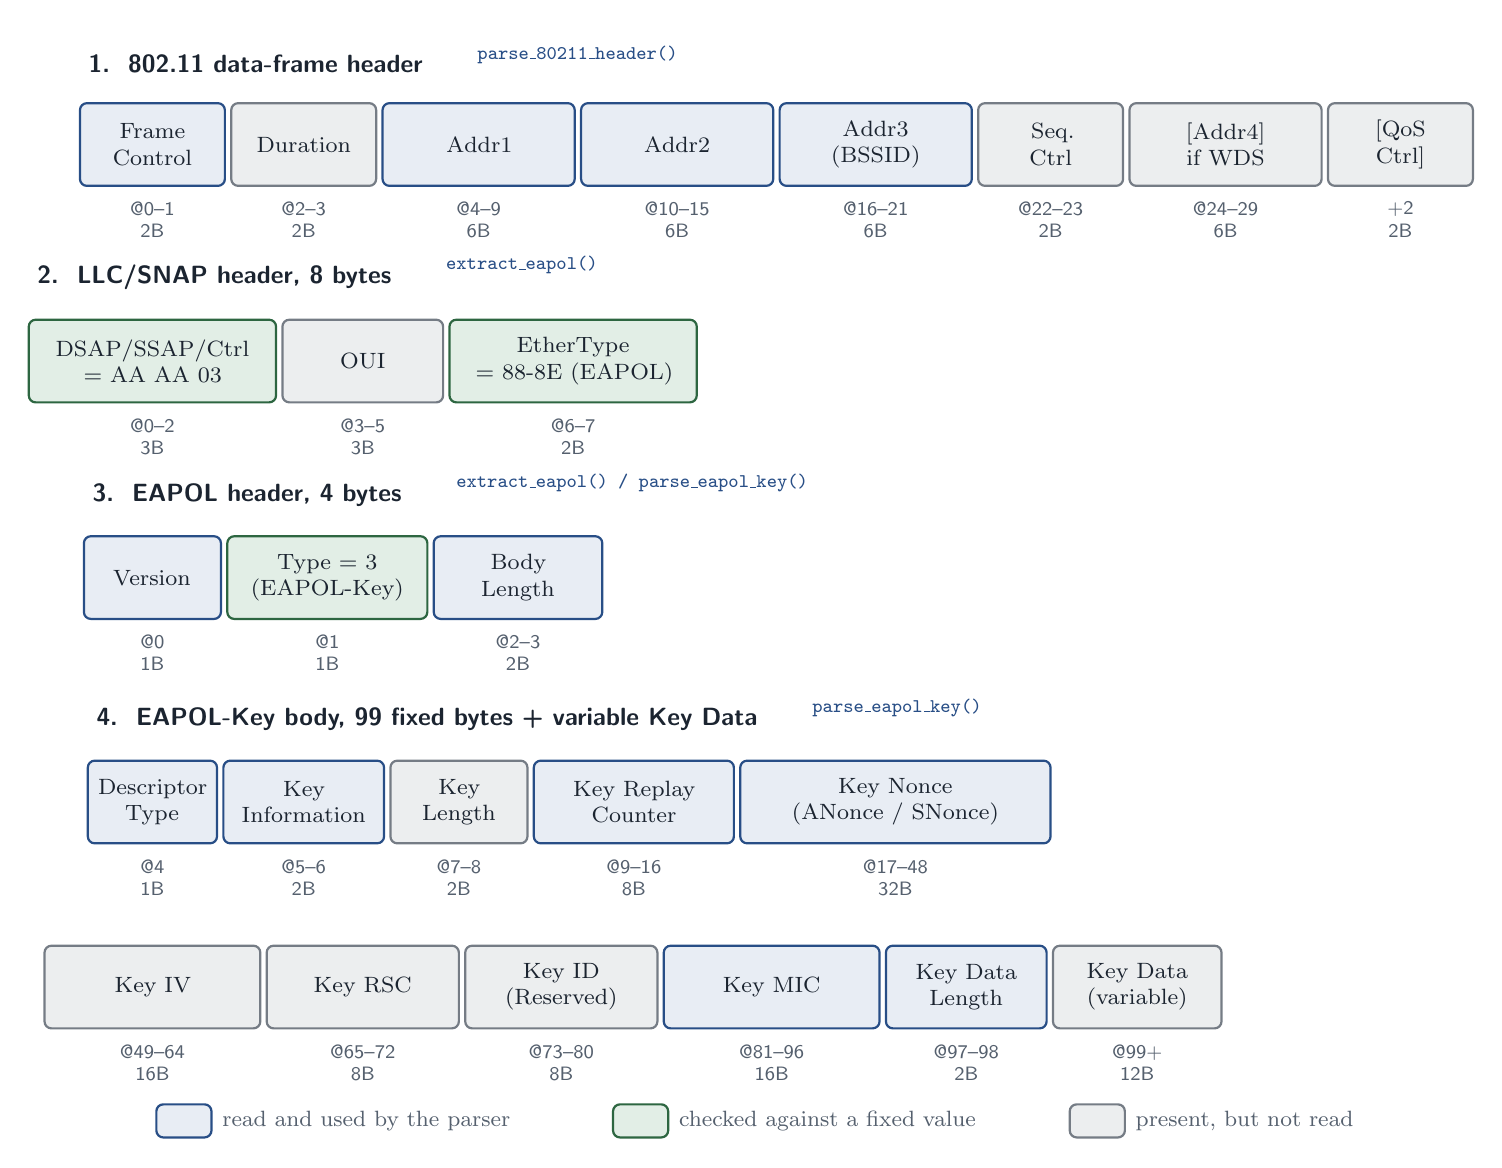
\begin{tikzpicture}
  \node[fR,text width=1.7cm] (a1) at (0,0) {Frame\\ Control};
  \node[fO,text width=1.7cm,right=1.5pt of a1] (a2) {Duration};
  \node[fR,text width=2.3cm,right=1.5pt of a2] (a3) {Addr1};
  \node[fR,text width=2.3cm,right=1.5pt of a3] (a4) {Addr2};
  \node[fR,text width=2.3cm,right=1.5pt of a4] (a5) {Addr3\\ (BSSID)};
  \node[fO,text width=1.7cm,right=1.5pt of a5] (a6) {Seq.\\ Ctrl};
  \node[fO,text width=2.3cm,right=1.5pt of a6] (a7) {[Addr4]\\ if WDS};
  \node[fO,text width=1.7cm,right=1.5pt of a7] (a8) {[QoS\\ Ctrl]};
  \node[ofl,below=2pt of a1]{@0--1\\2B};  \node[ofl,below=2pt of a2]{@2--3\\2B};
  \node[ofl,below=2pt of a3]{@4--9\\6B};  \node[ofl,below=2pt of a4]{@10--15\\6B};
  \node[ofl,below=2pt of a5]{@16--21\\6B};\node[ofl,below=2pt of a6]{@22--23\\2B};
  \node[ofl,below=2pt of a7]{@24--29\\6B};\node[ofl,below=2pt of a8]{+2\\2B};
  \node[sect] at ([yshift=7pt]a1.north west) {1.\ \ 802.11 data-frame header \ \ \ \ \tikz{\node[fn]{parse\_80211\_header()};}};
  \node[fG,text width=3.0cm] (b1) at (0,-2.75) {DSAP/SSAP/Ctrl\\ = AA AA 03};
  \node[fO,text width=1.9cm,right=1.5pt of b1] (b2) {OUI};
  \node[fG,text width=3.0cm,right=1.5pt of b2] (b3) {EtherType\\ = 88-8E (EAPOL)};
  \node[ofl,below=2pt of b1]{@0--2\\3B}; \node[ofl,below=2pt of b2]{@3--5\\3B}; \node[ofl,below=2pt of b3]{@6--7\\2B};
  \node[sect] at ([yshift=7pt]b1.north west) {2.\ \ LLC/SNAP header, 8 bytes \ \ \ \ \tikz{\node[fn]{extract\_eapol()};}};
  \node[fR,text width=1.6cm] (c1) at (0,-5.5) {Version};
  \node[fG,text width=2.4cm,right=1.5pt of c1] (c2) {Type = 3\\ (EAPOL-Key)};
  \node[fR,text width=2.0cm,right=1.5pt of c2] (c3) {Body\\ Length};
  \node[ofl,below=2pt of c1]{@0\\1B}; \node[ofl,below=2pt of c2]{@1\\1B}; \node[ofl,below=2pt of c3]{@2--3\\2B};
  \node[sect] at ([yshift=7pt]c1.north west) {3.\ \ EAPOL header, 4 bytes \ \ \ \ \tikz{\node[fn]{extract\_eapol() / parse\_eapol\_key()};}};
  \node[fR,text width=1.5cm] (d1) at (0,-8.35) {Descriptor\\ Type};
  \node[fR,text width=1.9cm,right=1.5pt of d1] (d2) {Key\\ Information};
  \node[fO,text width=1.6cm,right=1.5pt of d2] (d3) {Key\\ Length};
  \node[fR,text width=2.4cm,right=1.5pt of d3] (d4) {Key Replay\\ Counter};
  \node[fR,text width=3.8cm,right=1.5pt of d4] (d5) {Key Nonce\\ (ANonce / SNonce)};
  \node[ofl,below=2pt of d1]{@4\\1B}; \node[ofl,below=2pt of d2]{@5--6\\2B}; \node[ofl,below=2pt of d3]{@7--8\\2B};
  \node[ofl,below=2pt of d4]{@9--16\\8B}; \node[ofl,below=2pt of d5]{@17--48\\32B};
  \node[sect] at ([yshift=7pt]d1.north west) {4.\ \ EAPOL-Key body, 99 fixed bytes + variable Key Data \ \ \ \ \tikz{\node[fn]{parse\_eapol\_key()};}};
  \node[fO,text width=2.6cm] (e1) at (0,-10.7) {Key IV};
  \node[fO,text width=2.3cm,right=1.5pt of e1] (e2) {Key RSC};
  \node[fO,text width=2.3cm,right=1.5pt of e2] (e3) {Key ID\\ (Reserved)};
  \node[fR,text width=2.6cm,right=1.5pt of e3] (e4) {Key MIC};
  \node[fR,text width=1.9cm,right=1.5pt of e4] (e5) {Key Data\\ Length};
  \node[fO,text width=2.0cm,right=1.5pt of e5] (e6) {Key Data\\ (variable)};
  \node[ofl,below=2pt of e1]{@49--64\\16B}; \node[ofl,below=2pt of e2]{@65--72\\8B}; \node[ofl,below=2pt of e3]{@73--80\\8B};
  \node[ofl,below=2pt of e4]{@81--96\\16B}; \node[ofl,below=2pt of e5]{@97--98\\2B}; \node[ofl,below=2pt of e6]{@99+\\12B};
  \node[fR,minimum width=0.7cm,minimum height=0.42cm,text width=0.1cm] (lg1) at (0.4,-12.4) {};
  \node[anchor=west,font=\footnotesize,text=inksoft] at (lg1.east) {read and used by the parser};
  \node[fG,minimum width=0.7cm,minimum height=0.42cm,text width=0.1cm] (lg2) at (6.2,-12.4) {};
  \node[anchor=west,font=\footnotesize,text=inksoft] at (lg2.east) {checked against a fixed value};
  \node[fO,minimum width=0.7cm,minimum height=0.42cm,text width=0.1cm] (lg3) at (12.0,-12.4) {};
  \node[anchor=west,font=\footnotesize,text=inksoft] at (lg3.east) {present, but not read};
\end{tikzpicture}}
\caption{Frame encapsulation from the 802.11 header down to the EAPOL-Key body, with the exact byte offsets and field sizes used by the code. Offsets in layer~4 continue from byte~4 of the EAPOL frame.}
\label{fig:frame}
\end{figure}}

% ================= FIGURE 4 : KEY INFORMATION BITFIELD =================
\newcommand{\FIGFOUR}{%
\begin{figure}[!htb]\centering
\resizebox{\textwidth}{!}{%
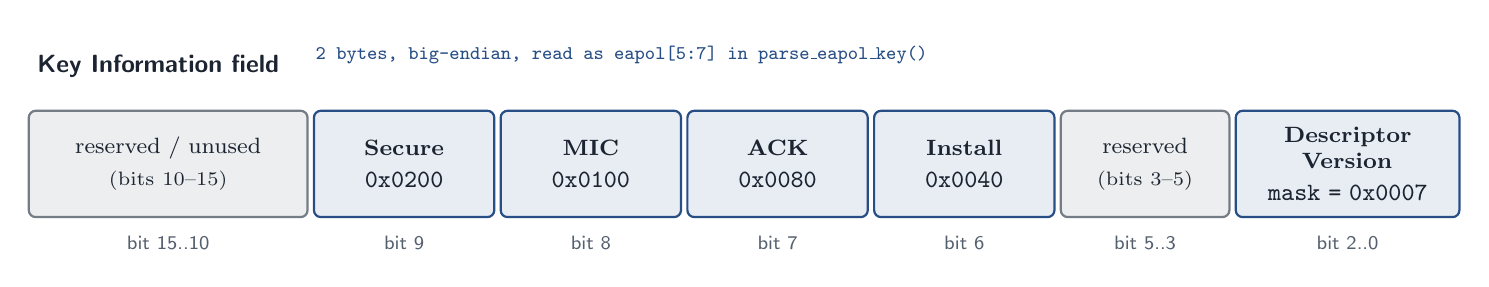
\begin{tikzpicture}
  \node[kO,text width=3.4cm] (k0) at (0,0) {reserved / unused\\[2pt]\scriptsize (bits 10--15)};
  \node[kR,text width=2.15cm,right=1.5pt of k0] (k1) {\textbf{Secure}\\[2pt]\code{0x0200}};
  \node[kR,text width=2.15cm,right=1.5pt of k1] (k2) {\textbf{MIC}\\[2pt]\code{0x0100}};
  \node[kR,text width=2.15cm,right=1.5pt of k2] (k3) {\textbf{ACK}\\[2pt]\code{0x0080}};
  \node[kR,text width=2.15cm,right=1.5pt of k3] (k4) {\textbf{Install}\\[2pt]\code{0x0040}};
  \node[kO,text width=2.0cm,right=1.5pt of k4] (k5) {reserved\\[2pt]\scriptsize (bits 3--5)};
  \node[kR,text width=2.7cm,right=1.5pt of k5] (k6) {\textbf{Descriptor Version}\\[2pt]\code{mask = 0x0007}};
  \foreach \n/\b in {k0/{bit 15..10},k1/{bit 9},k2/{bit 8},k3/{bit 7},k4/{bit 6},k5/{bit 5..3},k6/{bit 2..0}}
     \node[bitl,below=3pt of \n]{\b};
  \node[font=\sffamily\bfseries\small,text=ink,anchor=south west] at ([yshift=8pt]k0.north west)
     {Key Information field \ \ \tikz{\node[font=\ttfamily\scriptsize,text=accent!85!black]{2 bytes, big-endian, read as eapol[5:7] in parse\_eapol\_key()};}};
\end{tikzpicture}}
\caption{The Key Information bit field, decoded exactly as in \code{handshake.py}. \code{classify\_message()} names each message from these flags: \textbf{Msg 1} = ACK \& !MIC; \textbf{Msg 2} = MIC \& !ACK \& !Secure; \textbf{Msg 3} = ACK \& MIC \& Secure \& Install; \textbf{Msg 4} = MIC \& Secure \& !ACK \& !Install. Any other combination classifies as 0 and is ignored.}
\label{fig:keyinfo}
\end{figure}}

% ================= FIGURE 5 : PIPELINE FLOWCHART =================
\newcommand{\FIGFIVE}{%
\begin{figure}[!htb]\centering
\resizebox{0.99\textwidth}{!}{%
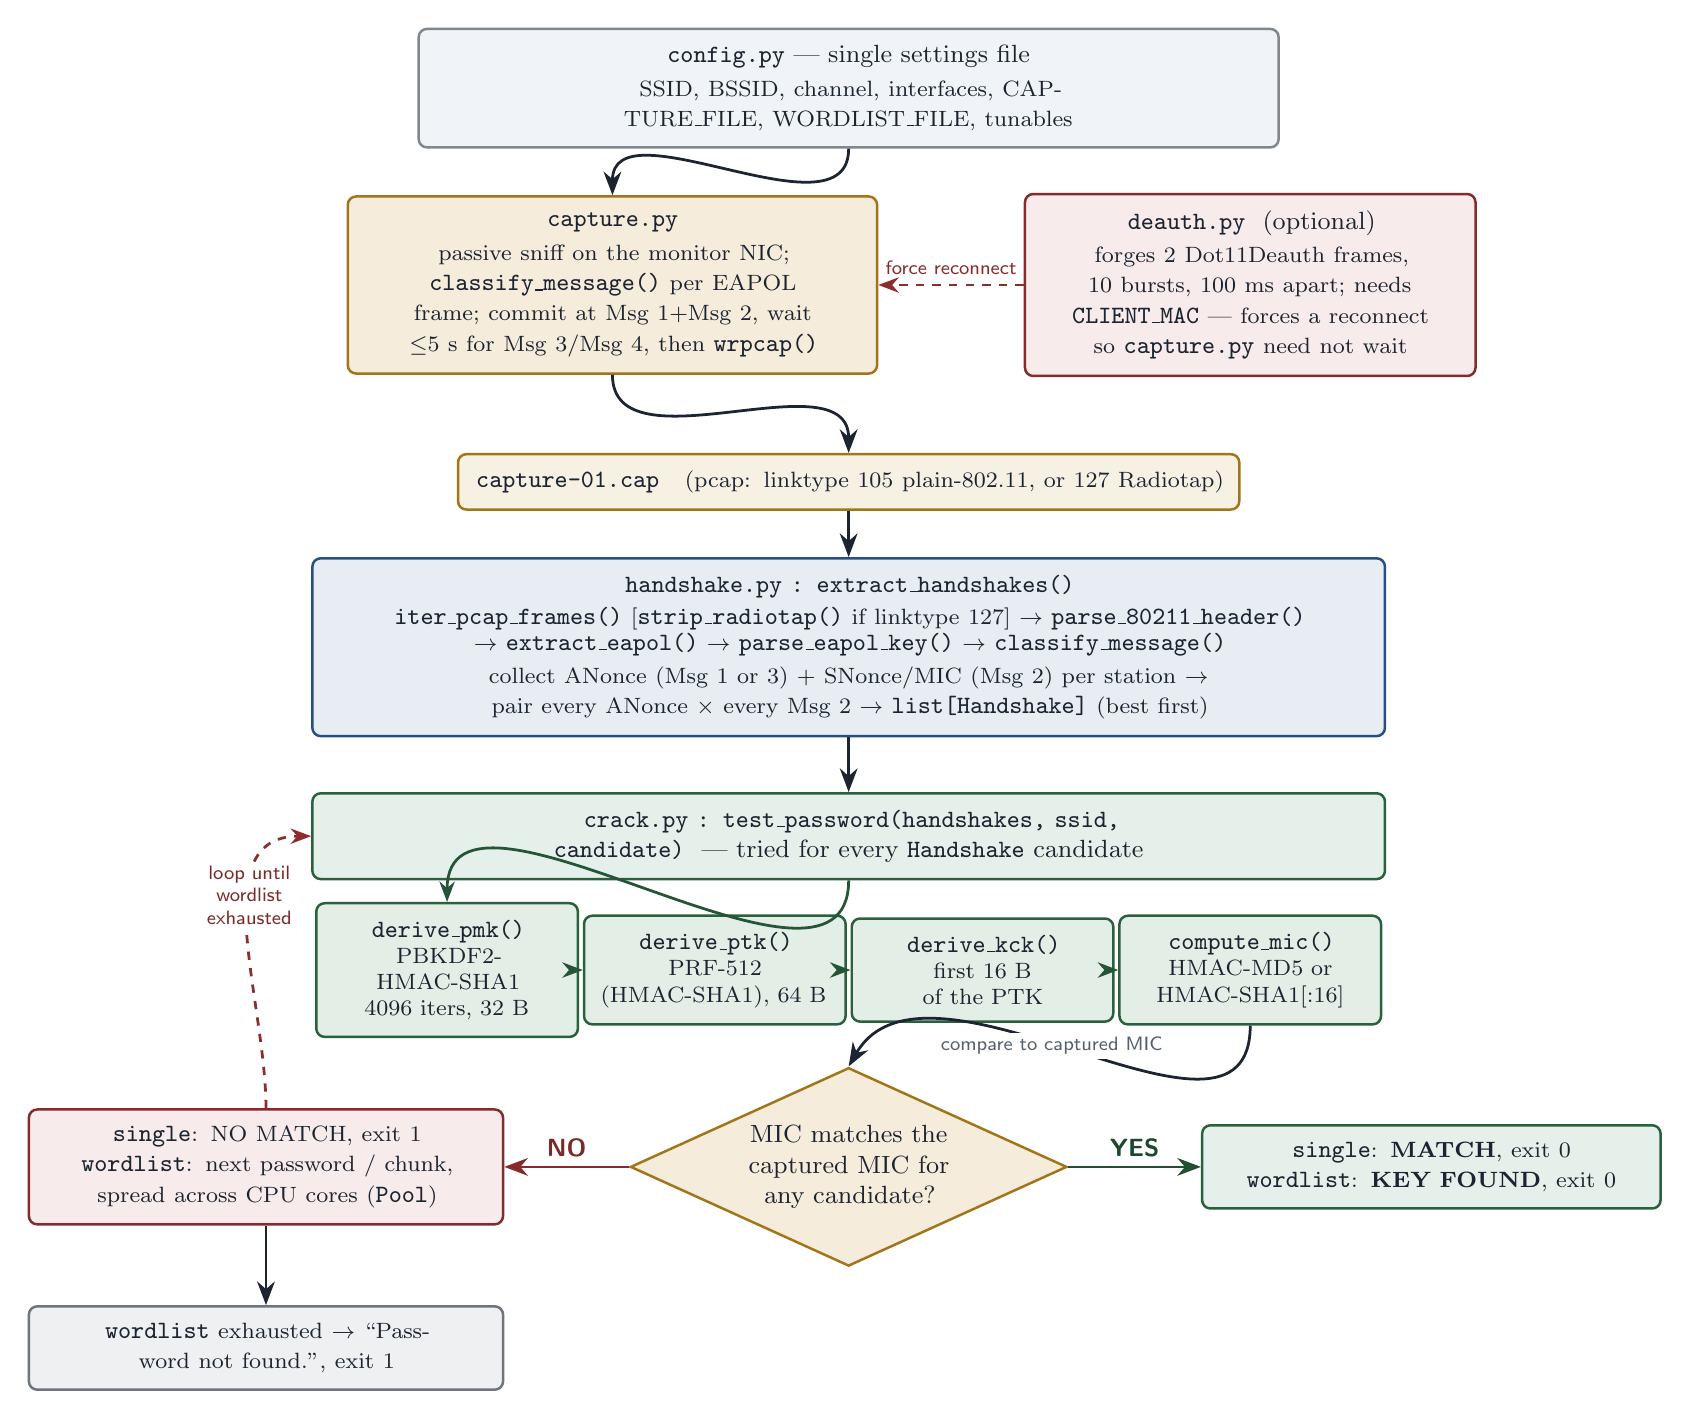
\begin{tikzpicture}
  \node[cfg,text width=10.5cm] (cfg) at (0,0)
     {\code{config.py} --- single settings file\\[1pt]\footnotesize SSID, BSSID, channel, interfaces, CAPTURE\_FILE, WORDLIST\_FILE, tunables};
  \node[snif,text width=6.3cm] (snif) at (-3.0,-2.5)
     {\code{capture.py}\\[1pt]\footnotesize passive sniff on the monitor NIC; \code{classify\_message()} per EAPOL frame; commit at Msg 1+Msg 2, wait $\leq$5 s for Msg 3/Msg 4, then \code{wrpcap()}};
  \node[deau,text width=5.3cm] (deau) at (5.1,-2.5)
     {\code{deauth.py} \ (optional)\\[1pt]\footnotesize forges 2 Dot11Deauth frames, 10 bursts, 100 ms apart; needs \code{CLIENT\_MAC} --- forces a reconnect so \code{capture.py} need not wait};
  \node[capf,text width=9.5cm] (capf) at (0,-5.0)
     {\code{capture-01.cap} \ \ \footnotesize(pcap: linktype 105 plain-802.11, or 127 Radiotap)};
  \node[hs,text width=13.2cm] (hs) at (0,-7.1)
     {\code{handshake.py : extract\_handshakes()}\\[2pt]\footnotesize \code{iter\_pcap\_frames()} [\code{strip\_radiotap()} if linktype 127] $\rightarrow$ \code{parse\_80211\_header()} $\rightarrow$ \code{extract\_eapol()} $\rightarrow$ \code{parse\_eapol\_key()} $\rightarrow$ \code{classify\_message()}\\[1pt]\footnotesize collect ANonce (Msg 1 or 3) + SNonce/MIC (Msg 2) per station $\rightarrow$ pair every ANonce $\times$ every Msg 2 $\rightarrow$ \code{list[Handshake]} (best first)};
  \node[cr,text width=13.2cm] (crk) at (0,-9.5)
     {\code{crack.py : test\_password(handshakes, ssid, candidate)} \ --- tried for every \code{Handshake} candidate};
  \node[cbox,text width=2.9cm] (c1) at (-5.1,-11.2){\code{derive\_pmk()}\\ PBKDF2-HMAC-SHA1\\ 4096 iters, 32 B};
  \node[cbox,text width=2.9cm] (c2) at (-1.7,-11.2){\code{derive\_ptk()}\\ PRF-512\\ (HMAC-SHA1), 64 B};
  \node[cbox,text width=2.9cm] (c3) at (1.7,-11.2){\code{derive\_kck()}\\ first 16 B\\ of the PTK};
  \node[cbox,text width=2.9cm] (c4) at (5.1,-11.2){\code{compute\_mic()}\\ HMAC-MD5 or\\ HMAC-SHA1[:16]};
  \node[dia,text width=3.0cm] (dia) at (0,-13.7){MIC matches the captured MIC for any candidate?};
  \node[cr,text width=5.4cm] (yes) at (7.4,-13.7)
     {\footnotesize\code{single}: \textbf{MATCH}, exit 0\\ \code{wordlist}: \textbf{KEY FOUND}, exit 0};
  \node[deau,text width=5.6cm] (no) at (-7.4,-13.7)
     {\footnotesize\code{single}: NO MATCH, exit 1\\ \code{wordlist}: next password / chunk, spread across CPU cores (\code{Pool})};
  \node[term,text width=5.6cm] (term) at (-7.4,-16.0)
     {\footnotesize\code{wordlist} exhausted $\rightarrow$ ``Password not found.'', exit 1};
  \draw[flow] (cfg.south) to[out=-90,in=90] (snif.north);
  \draw[flowred] (deau.west) -- node[lbl,above,text=red!75!black]{force reconnect} (snif.east);
  \draw[flow] (snif.south) to[out=-90,in=90] (capf.north);
  \draw[flow] (capf.south) -- (hs.north);
  \draw[flow] (hs.south) -- (crk.north);
  \draw[fg] (crk.south) to[out=-90,in=90] (c1.north);
  \draw[fg] (c1.east) -- (c2.west);
  \draw[fg] (c2.east) -- (c3.west);
  \draw[fg] (c3.east) -- (c4.west);
  \draw[flow] (c4.south) to[out=-90,in=60] node[lbl,text=inksoft,pos=0.55,fill=white,inner sep=1.5pt]{compare to captured MIC} (dia.north);
  \draw[flow,draw=green!55!black] (dia.east) -- node[lbl,above,text=green!50!black,font=\sffamily\bfseries\small]{YES} (yes.west);
  \draw[flow,draw=red!75!black] (dia.west) -- node[lbl,above,text=red!70!black,font=\sffamily\bfseries\small]{NO} (no.east);
  \draw[flow] (no.south) -- (term.north);
  \draw[flowred] (no.north) to[out=90,in=180]
        node[lbl,text=red!70!black,pos=0.62,fill=white,inner sep=1.5pt,align=center]{loop until\\ wordlist\\ exhausted} (crk.west);
\end{tikzpicture}}
\caption{The implementation pipeline, from \code{config.py} through to a \textsc{match} / \textsc{no match} decision. The four green boxes are the from-scratch crypto chain inside \code{test\_password()}; the dashed loop returns to \code{crack.py} for the next candidate until the wordlist is exhausted.}
\label{fig:pipeline}
\end{figure}}

% ================= FIGURE 6 : WHY THE OFFLINE ATTACK DIES UNDER SAE =================
\newcommand{\FIGSIX}{%
\begin{figure}[H]\centering
\resizebox{0.86\textwidth}{!}{%
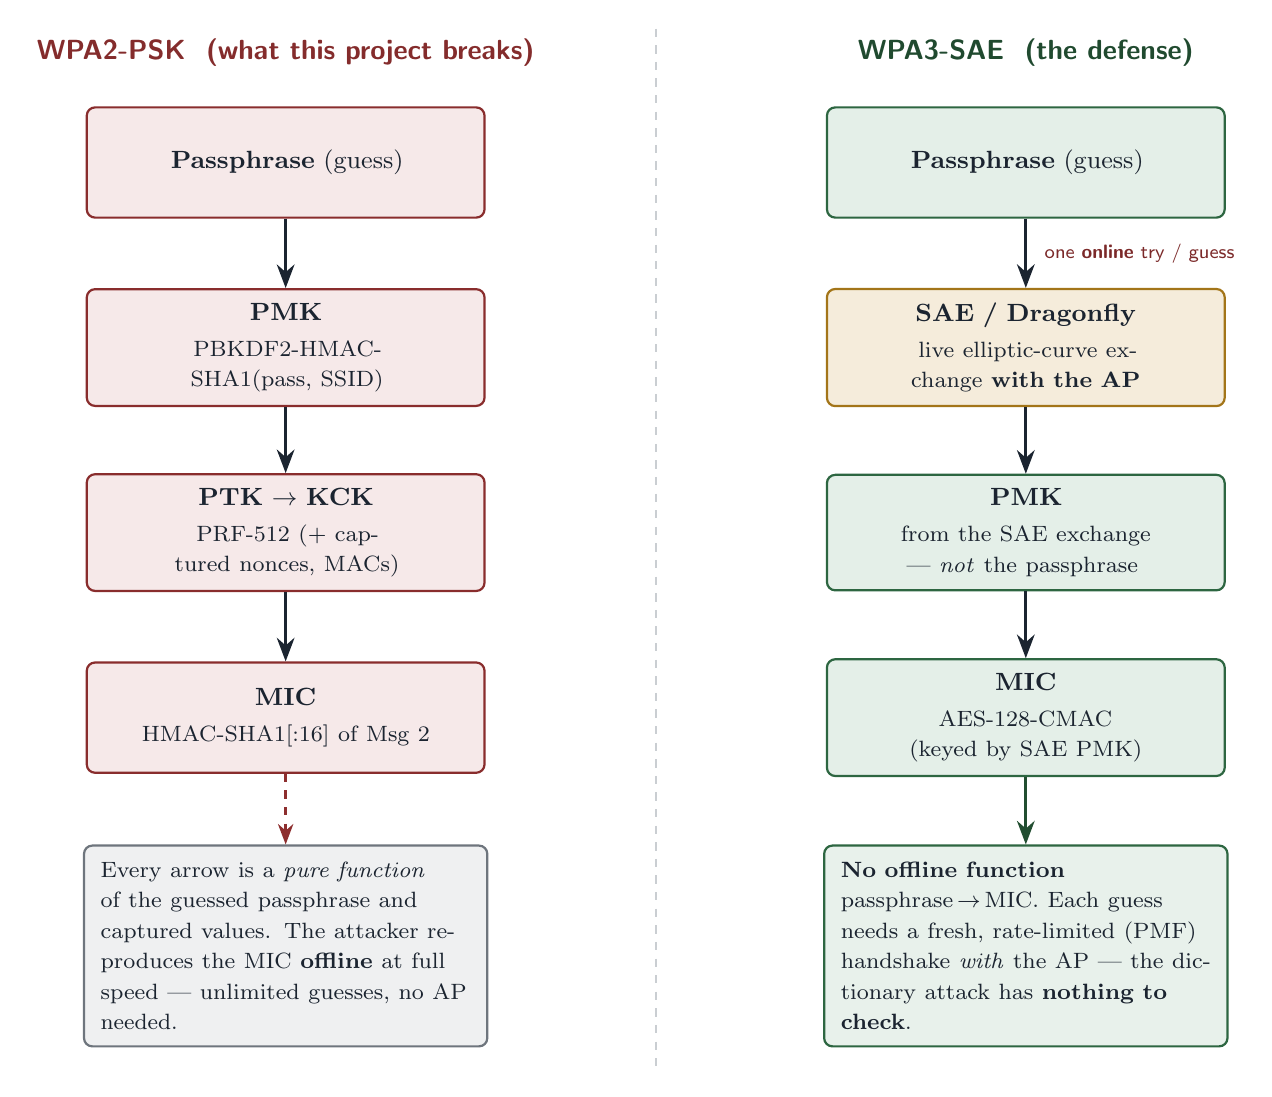
\begin{tikzpicture}[font=\small,node distance=0pt]
  \def\lx{-4.7}\def\rx{4.7}
  \def\ya{0}\def\yb{-2.35}\def\yc{-4.7}\def\yd{-7.05}
  \tikzset{chain/.style={rounded corners=3pt,align=center,inner sep=5pt,line width=0.8pt,
      text width=4.7cm,minimum height=1.4cm,text=ink},
    note/.style={rounded corners=3pt,align=left,inner sep=6pt,line width=0.8pt,
      text width=4.7cm,text=ink}}
  % --- column headers ---
  \node[font=\sffamily\bfseries,text=red!75!black] at (\lx,1.4) {WPA2-PSK\ \ (what this project breaks)};
  \node[font=\sffamily\bfseries,text=green!52!black] at (\rx,1.4) {WPA3-SAE\ \ (the defense)};
  % --- LEFT: WPA2 chain ---
  \node[chain,fill=red!11,draw=red!78!black] (lp) at (\lx,\ya) {\textbf{Passphrase} (guess)};
  \node[chain,fill=red!11,draw=red!78!black] (l1) at (\lx,\yb) {\textbf{PMK}\\[2pt]\footnotesize PBKDF2-HMAC-SHA1(pass, SSID)};
  \node[chain,fill=red!11,draw=red!78!black] (l2) at (\lx,\yc) {\textbf{PTK $\rightarrow$ KCK}\\[2pt]\footnotesize PRF-512 (+ captured nonces, MACs)};
  \node[chain,fill=red!11,draw=red!78!black] (l3) at (\lx,\yd) {\textbf{MIC}\\[2pt]\footnotesize HMAC-SHA1$[{:}16]$ of Msg 2};
  \draw[flow] (lp.south) -- (l1.north);
  \draw[flow] (l1.south) -- (l2.north);
  \draw[flow] (l2.south) -- (l3.north);
  \node[note,fill=gray!14,draw=gray!80!black] (lnote) at (\lx,-9.95)
     {\footnotesize Every arrow is a \emph{pure function} of the guessed passphrase and captured values. The attacker reproduces the MIC \textbf{offline} at full speed --- unlimited guesses, no AP needed.};
  \draw[flowred] (l3.south) -- (lnote.north);
  % --- RIGHT: WPA3 chain ---
  \node[chain,fill=green!14,draw=green!72!black] (rp) at (\rx,\ya) {\textbf{Passphrase} (guess)};
  \node[chain,fill=amber!16,draw=amber!85!black] (r1) at (\rx,\yb) {\textbf{SAE / Dragonfly}\\[2pt]\footnotesize live elliptic-curve exchange \textbf{with the AP}};
  \node[chain,fill=green!14,draw=green!72!black] (r2) at (\rx,\yc) {\textbf{PMK}\\[2pt]\footnotesize from the SAE exchange --- \emph{not} the passphrase};
  \node[chain,fill=green!14,draw=green!72!black] (r3) at (\rx,\yd) {\textbf{MIC}\\[2pt]\footnotesize AES-128-CMAC (keyed by SAE PMK)};
  \draw[flow] (rp.south) -- node[lbl,right=3pt,text=red!70!black]{one \textbf{online} try / guess} (r1.north);
  \draw[flow] (r1.south) -- (r2.north);
  \draw[flow] (r2.south) -- (r3.north);
  \node[note,fill=green!12,draw=green!72!black] (rnote) at (\rx,-9.95)
     {\footnotesize \textbf{No offline function} passphrase\,$\rightarrow$\,MIC. Each guess needs a fresh, rate-limited (PMF) handshake \emph{with} the AP --- the dictionary attack has \textbf{nothing to check}.};
  \draw[flow,draw=green!55!black] (r3.south) -- (rnote.north);
  % --- divider ---
  \draw[gray!45,line width=0.7pt,dashed] (0,1.7) -- (0,-11.5);
\end{tikzpicture}}
\caption{The same offline attack, side by side, against WPA2-PSK and WPA3-SAE. In WPA2 the whole PMK\,$\rightarrow$\,PTK\,$\rightarrow$\,MIC chain is a deterministic function of the guessed passphrase, so it can be replayed offline (left). In WPA3-SAE the PMK is produced by a \emph{live} elliptic-curve exchange with the AP, so no captured transcript lets an attacker turn a passphrase guess into the captured MIC (right) --- the vulnerability is removed at the root, not merely hidden.}
\label{fig:sae}
\end{figure}}

% ================= FIGURE 7 : SAE + PMF TIMING =================
\newcommand{\FIGSEVEN}{%
\begin{figure}[H]\centering
\resizebox{0.95\textwidth}{!}{%
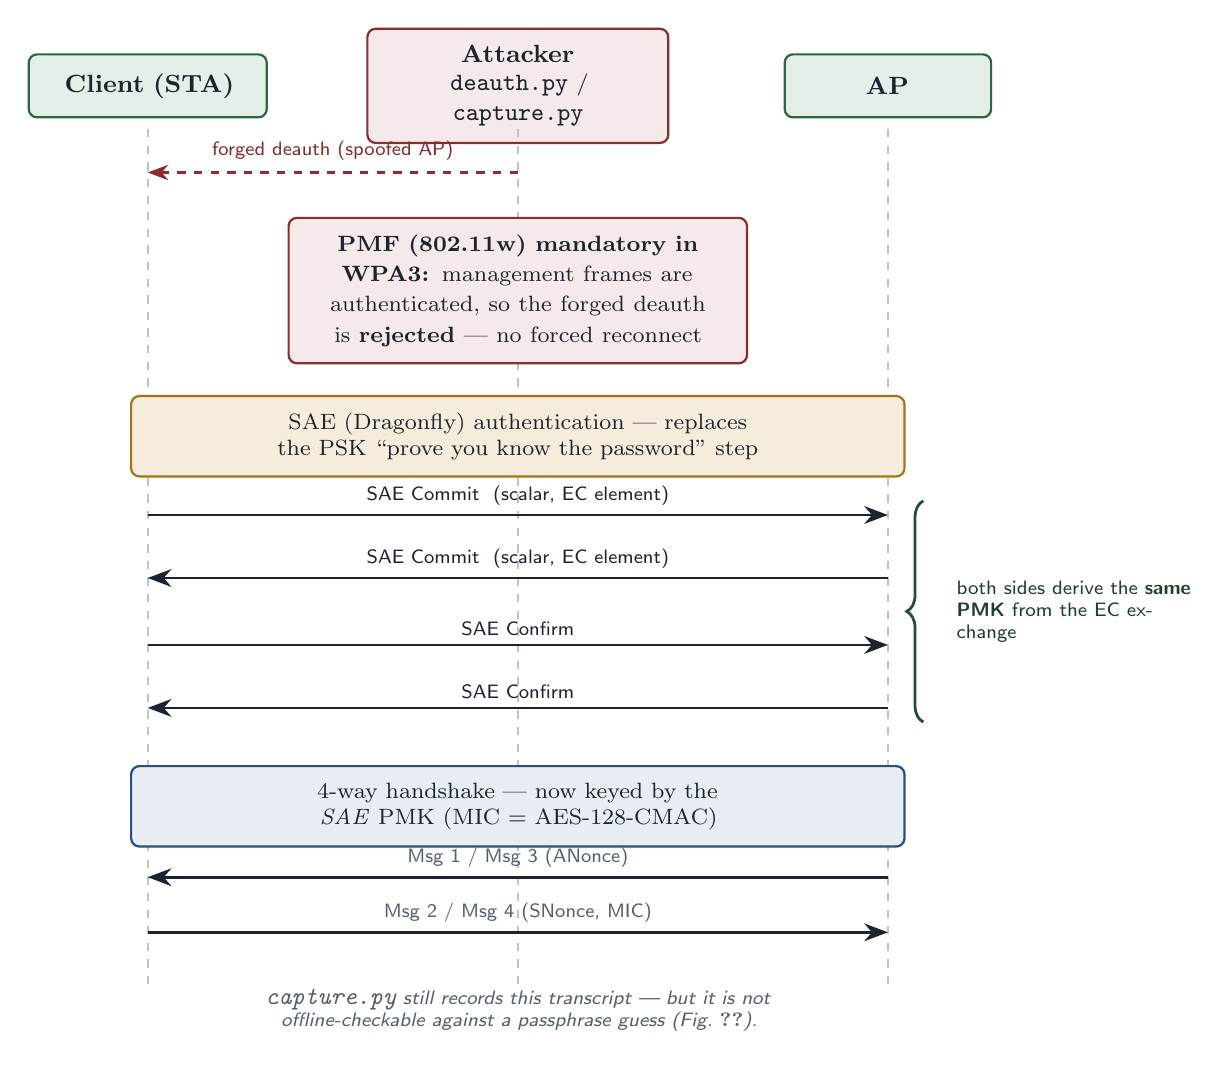
\begin{tikzpicture}[font=\small]
  \def\sta{0}\def\att{4.7}\def\ap{9.4}
  \def\ybot{-11.5}
  \node[bChk,text width=2.6cm,minimum height=0.8cm] (hSTA) at (\sta,0) {\textbf{Client (STA)}};
  \node[bRed,text width=3.4cm,minimum height=0.8cm] (hATT) at (\att,0) {\textbf{Attacker}\\[-1pt]\footnotesize \code{deauth.py} / \code{capture.py}};
  \node[bChk,text width=2.2cm,minimum height=0.8cm] (hAP)  at (\ap,0)  {\textbf{AP}};
  \foreach \x in {\sta,\att,\ap} \draw[gray!55,dashed,line width=0.7pt] (\x,-0.55) -- (\x,\ybot);
  % --- forged deauth blocked by PMF ---
  \draw[flowred] (\att,-1.1) -- (\sta,-1.1);
  \node[lbl,text=red!75!black,above=0pt] at ({(\att+\sta)/2},-1.07) {forged deauth (spoofed AP)};
  \node[bRed,text width=5.4cm,align=center] at (\att,-2.6)
     {\footnotesize \textbf{PMF (802.11w) mandatory in WPA3:} management frames are authenticated, so the forged deauth is \textbf{rejected} --- no forced reconnect};
  % --- SAE section ---
  \node[bAmber,text width=9.4cm,minimum height=0.55cm,font=\footnotesize] (sae) at ({(\sta+\ap)/2},-4.45)
     {SAE (Dragonfly) authentication --- replaces the PSK ``prove you know the password'' step};
  \def\ca{-5.45}\def\cb{-6.25}\def\cc{-7.1}\def\cd{-7.9}
  \draw[flow] (\sta,\ca) -- (\ap,\ca);
  \node[lbl,text=ink,above=0pt] at ({(\sta+\ap)/2},\ca) {SAE Commit\ \ (scalar, EC element)};
  \draw[flow] (\ap,\cb) -- (\sta,\cb);
  \node[lbl,text=ink,above=0pt] at ({(\sta+\ap)/2},\cb) {SAE Commit\ \ (scalar, EC element)};
  \draw[flow] (\sta,\cc) -- (\ap,\cc);
  \node[lbl,text=ink,above=0pt] at ({(\sta+\ap)/2},\cc) {SAE Confirm};
  \draw[flow] (\ap,\cd) -- (\sta,\cd);
  \node[lbl,text=ink,above=0pt] at ({(\sta+\ap)/2},\cd) {SAE Confirm};
  \draw[decorate,decoration={brace,mirror,amplitude=6pt},line width=1pt,green!55!black]
       (\ap+0.45,\ca+0.18) -- (\ap+0.45,\cd-0.18);
  \node[lbl,text=green!45!black,align=left,anchor=west,text width=3.0cm] at (\ap+0.75,{(\ca+\cd)/2})
       {both sides derive the \textbf{same PMK} from the EC exchange};
  % --- 4-way handshake keyed by SAE PMK ---
  \node[bRead,text width=9.4cm,minimum height=0.5cm,font=\footnotesize] (fw) at ({(\sta+\ap)/2},-9.15)
     {4-way handshake --- now keyed by the \emph{SAE} PMK (MIC = AES-128-CMAC)};
  \draw[flow] (\ap,-10.05) -- (\sta,-10.05);
  \node[lbl,above=0pt] at ({(\sta+\ap)/2},-10.05) {Msg 1 / Msg 3 (ANonce)};
  \draw[flow] (\sta,-10.75) -- (\ap,-10.75);
  \node[lbl,above=0pt] at ({(\sta+\ap)/2},-10.75) {Msg 2 / Msg 4 (SNonce, MIC)};
  \node[lbl,text=inksoft,align=center,anchor=north,text width=10.5cm] at ({(\sta+\ap)/2},-11.35)
     {\itshape \code{capture.py} still records this transcript --- but it is not offline-checkable against a passphrase guess (Fig.~\ref{fig:sae}).};
\end{tikzpicture}}
\caption{WPA3-SAE with mandatory PMF. The forged deauthentication frame \code{deauth.py} relies on is rejected as unauthenticated (top). Authentication is then done by the SAE Commit/Confirm exchange, whose PMK comes from live elliptic-curve material; the subsequent 4-way handshake is keyed by that PMK, so the captured handshake carries nothing an offline dictionary attack can test.}
\label{fig:saetiming}
\end{figure}}
